\documentclass[12pt,letterpaper]{article}
\usepackage[margin=1in]{geometry}
\usepackage{graphicx}
\usepackage{subfig}
\usepackage{color}
\usepackage{enumerate}
\usepackage{mathtools}
%\usepackage{amsfonts}
%\usepackage{amssymb}
%\usepackage{MnSymbol}
\usepackage{amsmath}
\usepackage{amsthm}
\usepackage{commath}

% Common parenthetic remarks
\newcommand{\ie}[1]             {(\textit{i.e.} #1)}
\newcommand{\eg}[1]             {(\textit{e.g.} #1)}

\newcommand{\N}					{{\mathbb N}}
\newcommand{\Z}					{{\mathbb Z}}
\newcommand{\Q}					{{\mathbb Q}}
\newcommand{\R}					{{\mathbb R}}
\newcommand{\C}					{{\mathbb C}}
\newcommand{\F}					{{\mathbb F}}
\newcommand{\T}					{{\mathbb T}}

% Macro for defining space in integral between integrand and infinitesimal
\renewcommand{\d}{\,d}

\newcommand{\gradient}[1]       {\vec{\nabla}#1}

% Distinguish bars in code
\newcommand{\conj}[1]			{\overline{#1}}
\newcommand{\mean}[1]			{\overline{#1}}

% I like operator form rather than weird font
\renewcommand{\Re}[1]			{\operatorname{Re}\left(#1\right)}
\renewcommand{\Im}[1]			{\operatorname{Im}\left(#1\right)}

% Set complement
\newcommand{\stcomp}[1]		   	{{#1}^\mathsf{c}}
\newcommand{\closure}[1]		{\overline{#1}}

% Directional derivative
\newcommand{\dirderiv}[2]       {\vec{\nabla}#1\cdot \hat{#2}}  

\newcommand\supp                {\mathop{\rm supp}}
\newcommand\sign[1]             {\mathop{\rm sgn}\del{#1}}

\DeclarePairedDelimiter{\ceil}{\lceil}{\rceil}

\newcommand\unitvec[1]          {\vec{\hat{#1}}}
\renewcommand\vec[1]            {\mathbf{#1}}

\begin{document}
% No automatic indenting
\setlength{\parindent}{0pt}

\begin{figure}[!hp]
\begin{center}
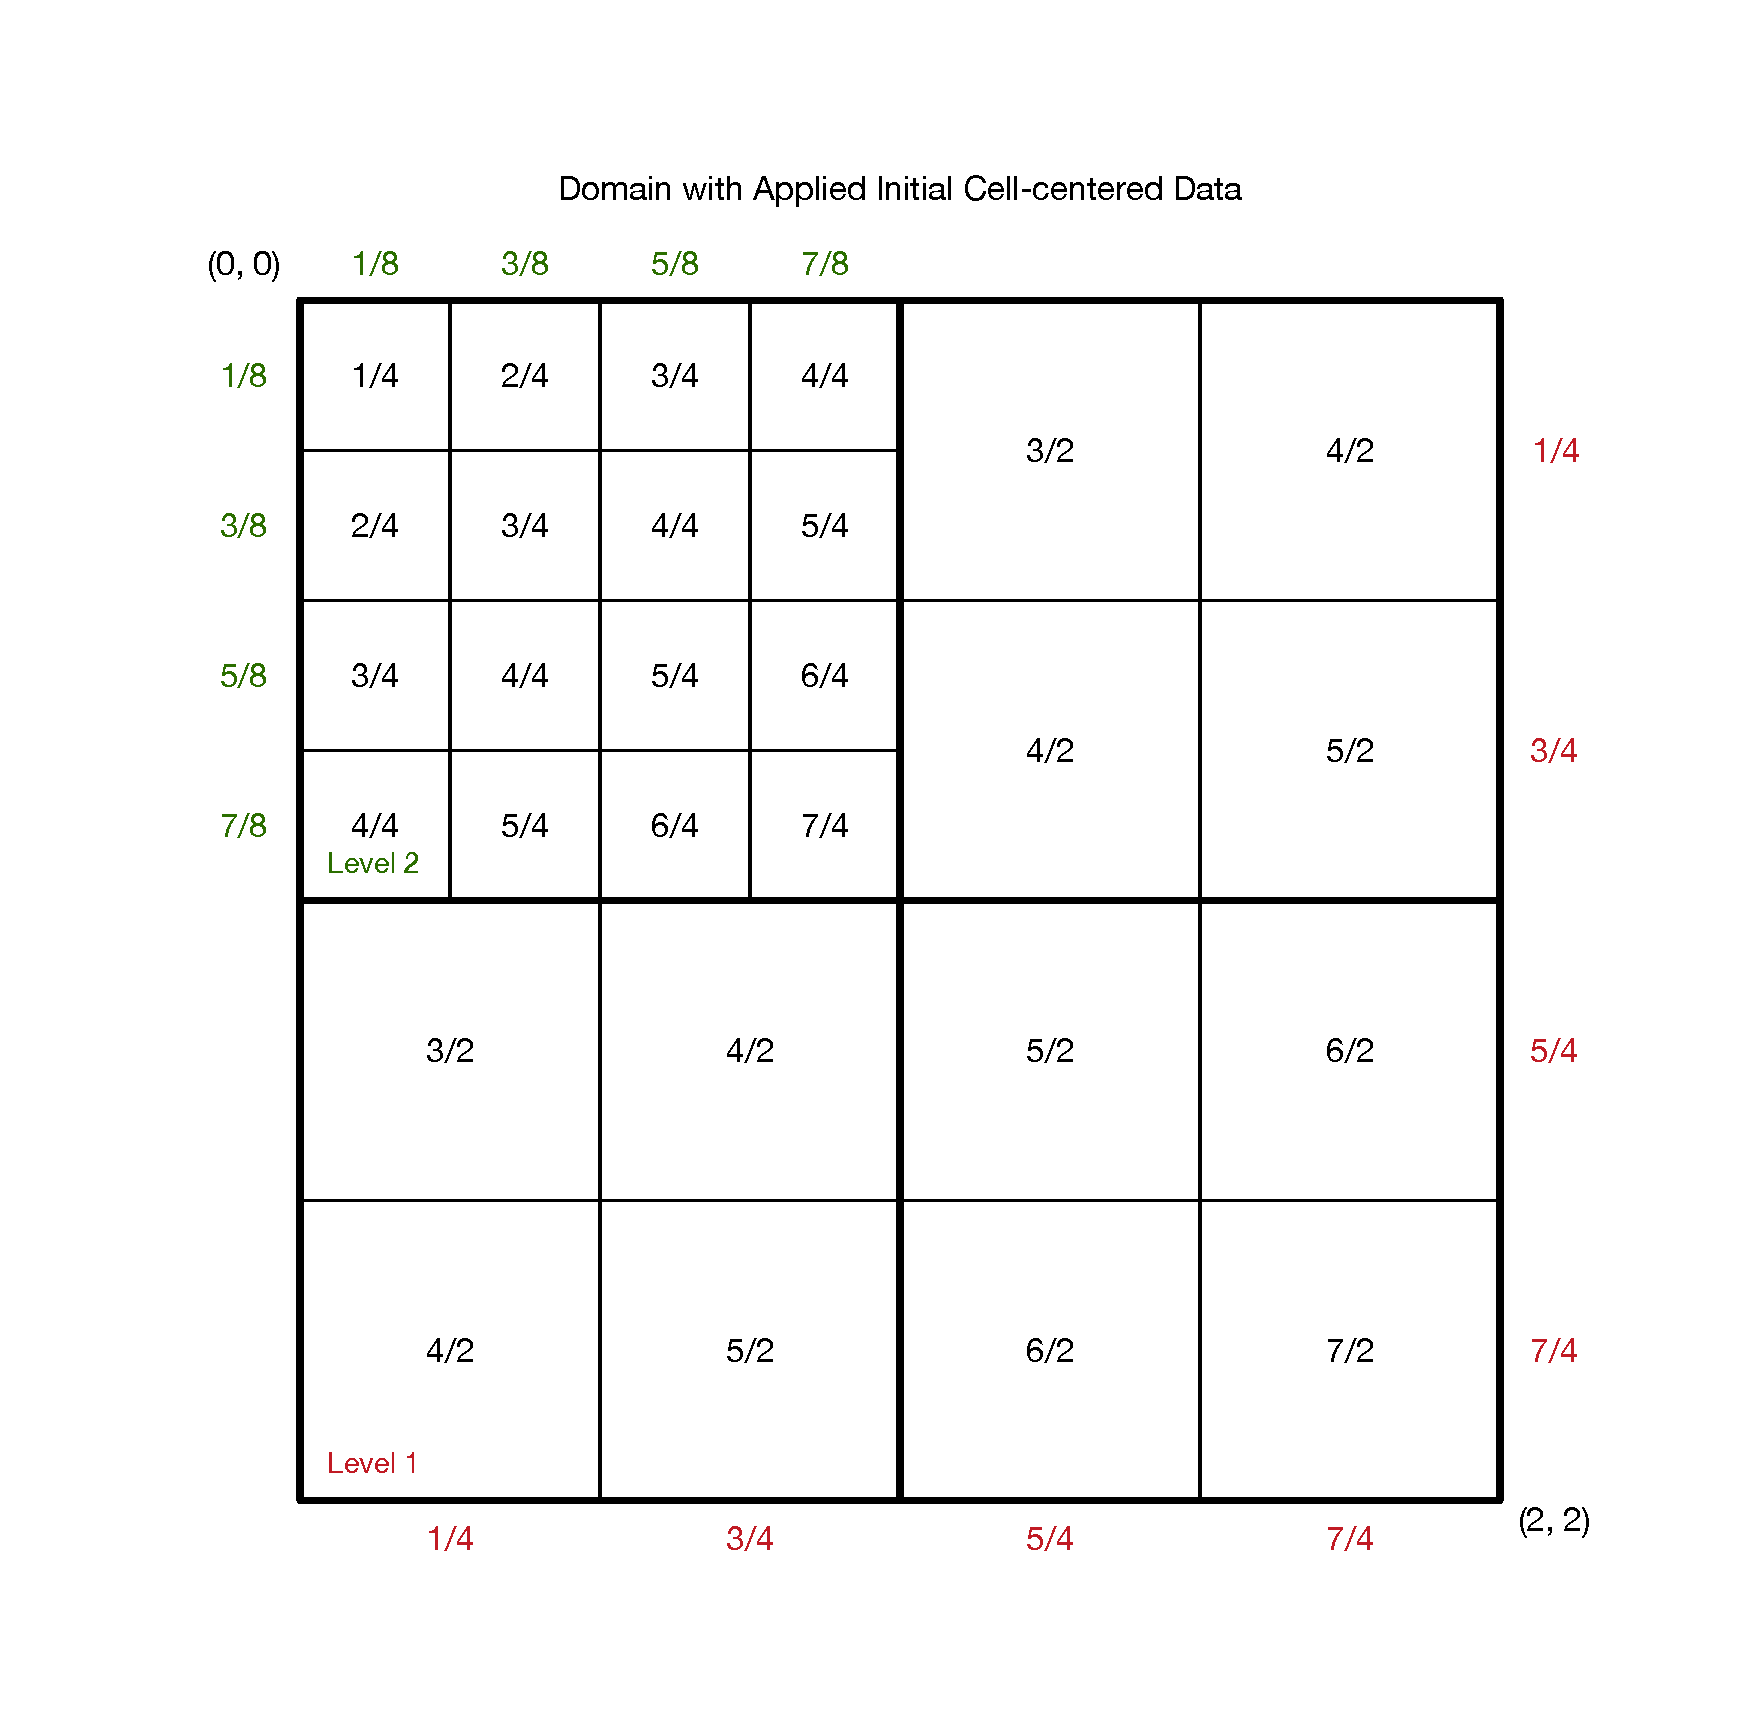
\includegraphics[width=6.5in]{TestGcFill_Domain.pdf}
\caption{The domain partitioned into blocks belonging to only two levels.  This
structure and the cell-centered data remain static during the unittest.}
\end{center}
\end{figure}

\newpage
\begin{figure}[!hp]
\begin{center}
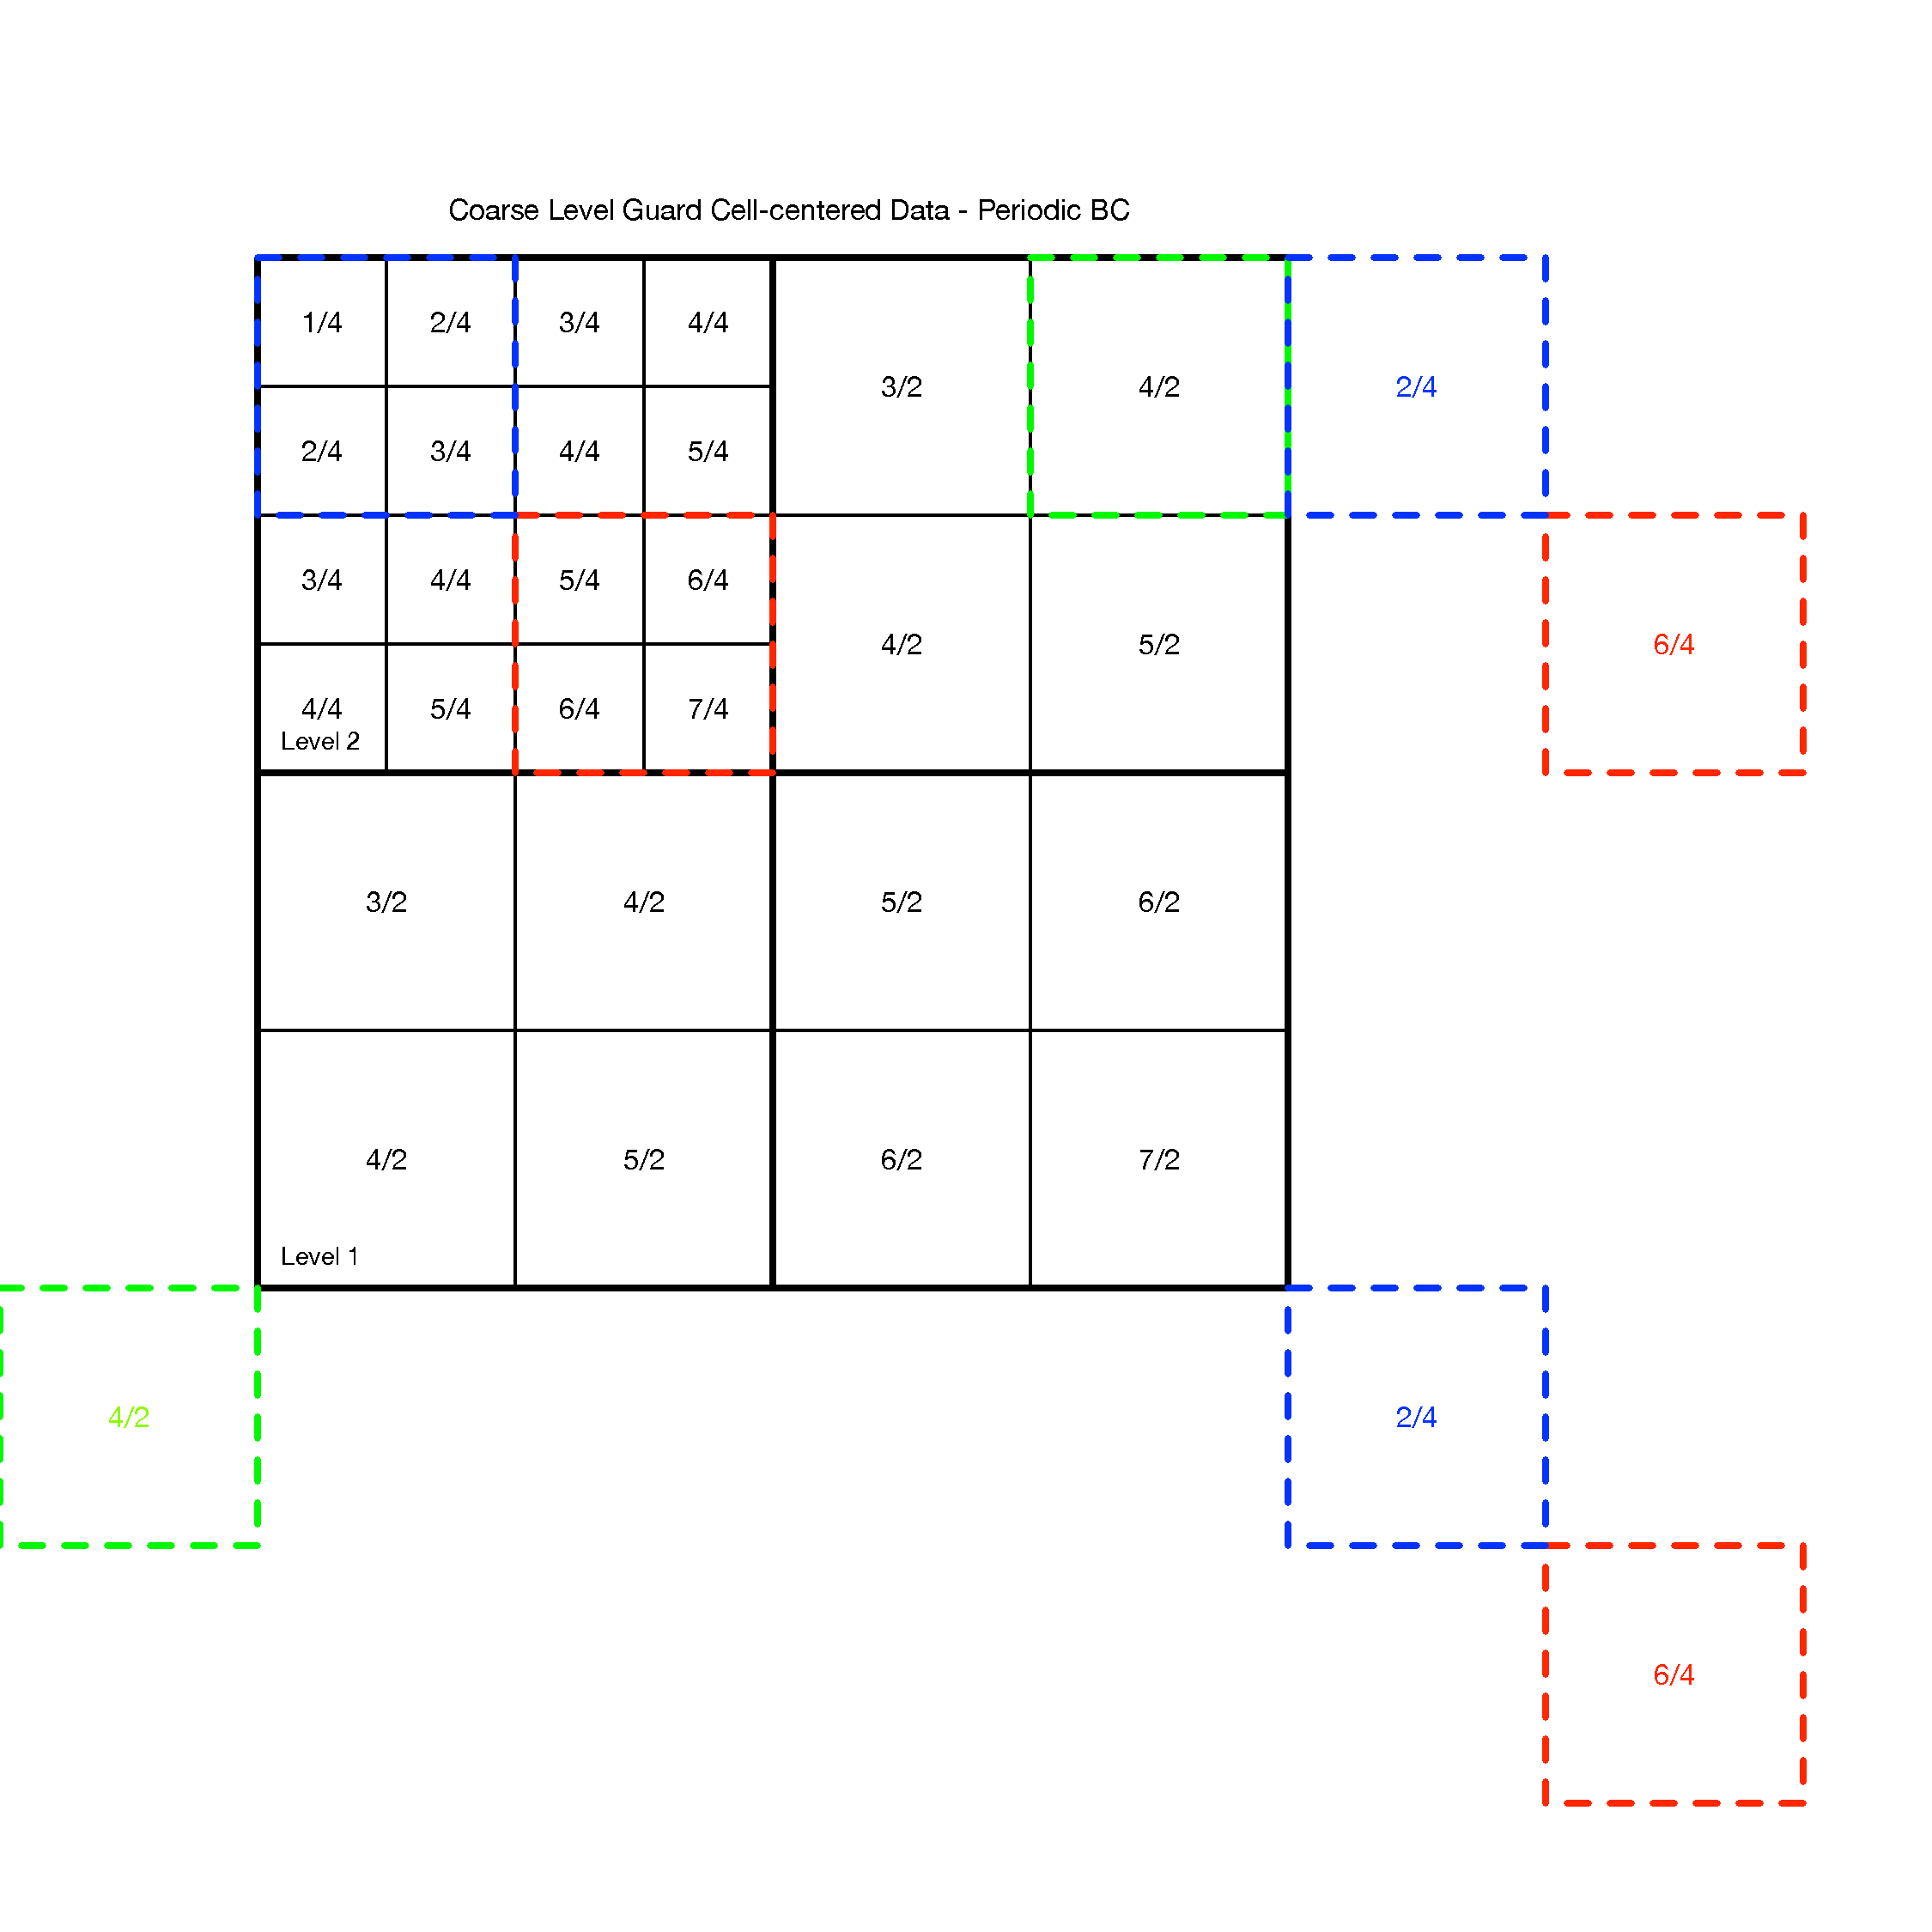
\includegraphics[width=6.5in]{TestGcFill_CoarseGC.pdf}
\caption{Spot check some cell-centered guardcell data in Level 1.}
\end{center}
\end{figure}

\newpage
\begin{figure}[!hp]
\begin{center}
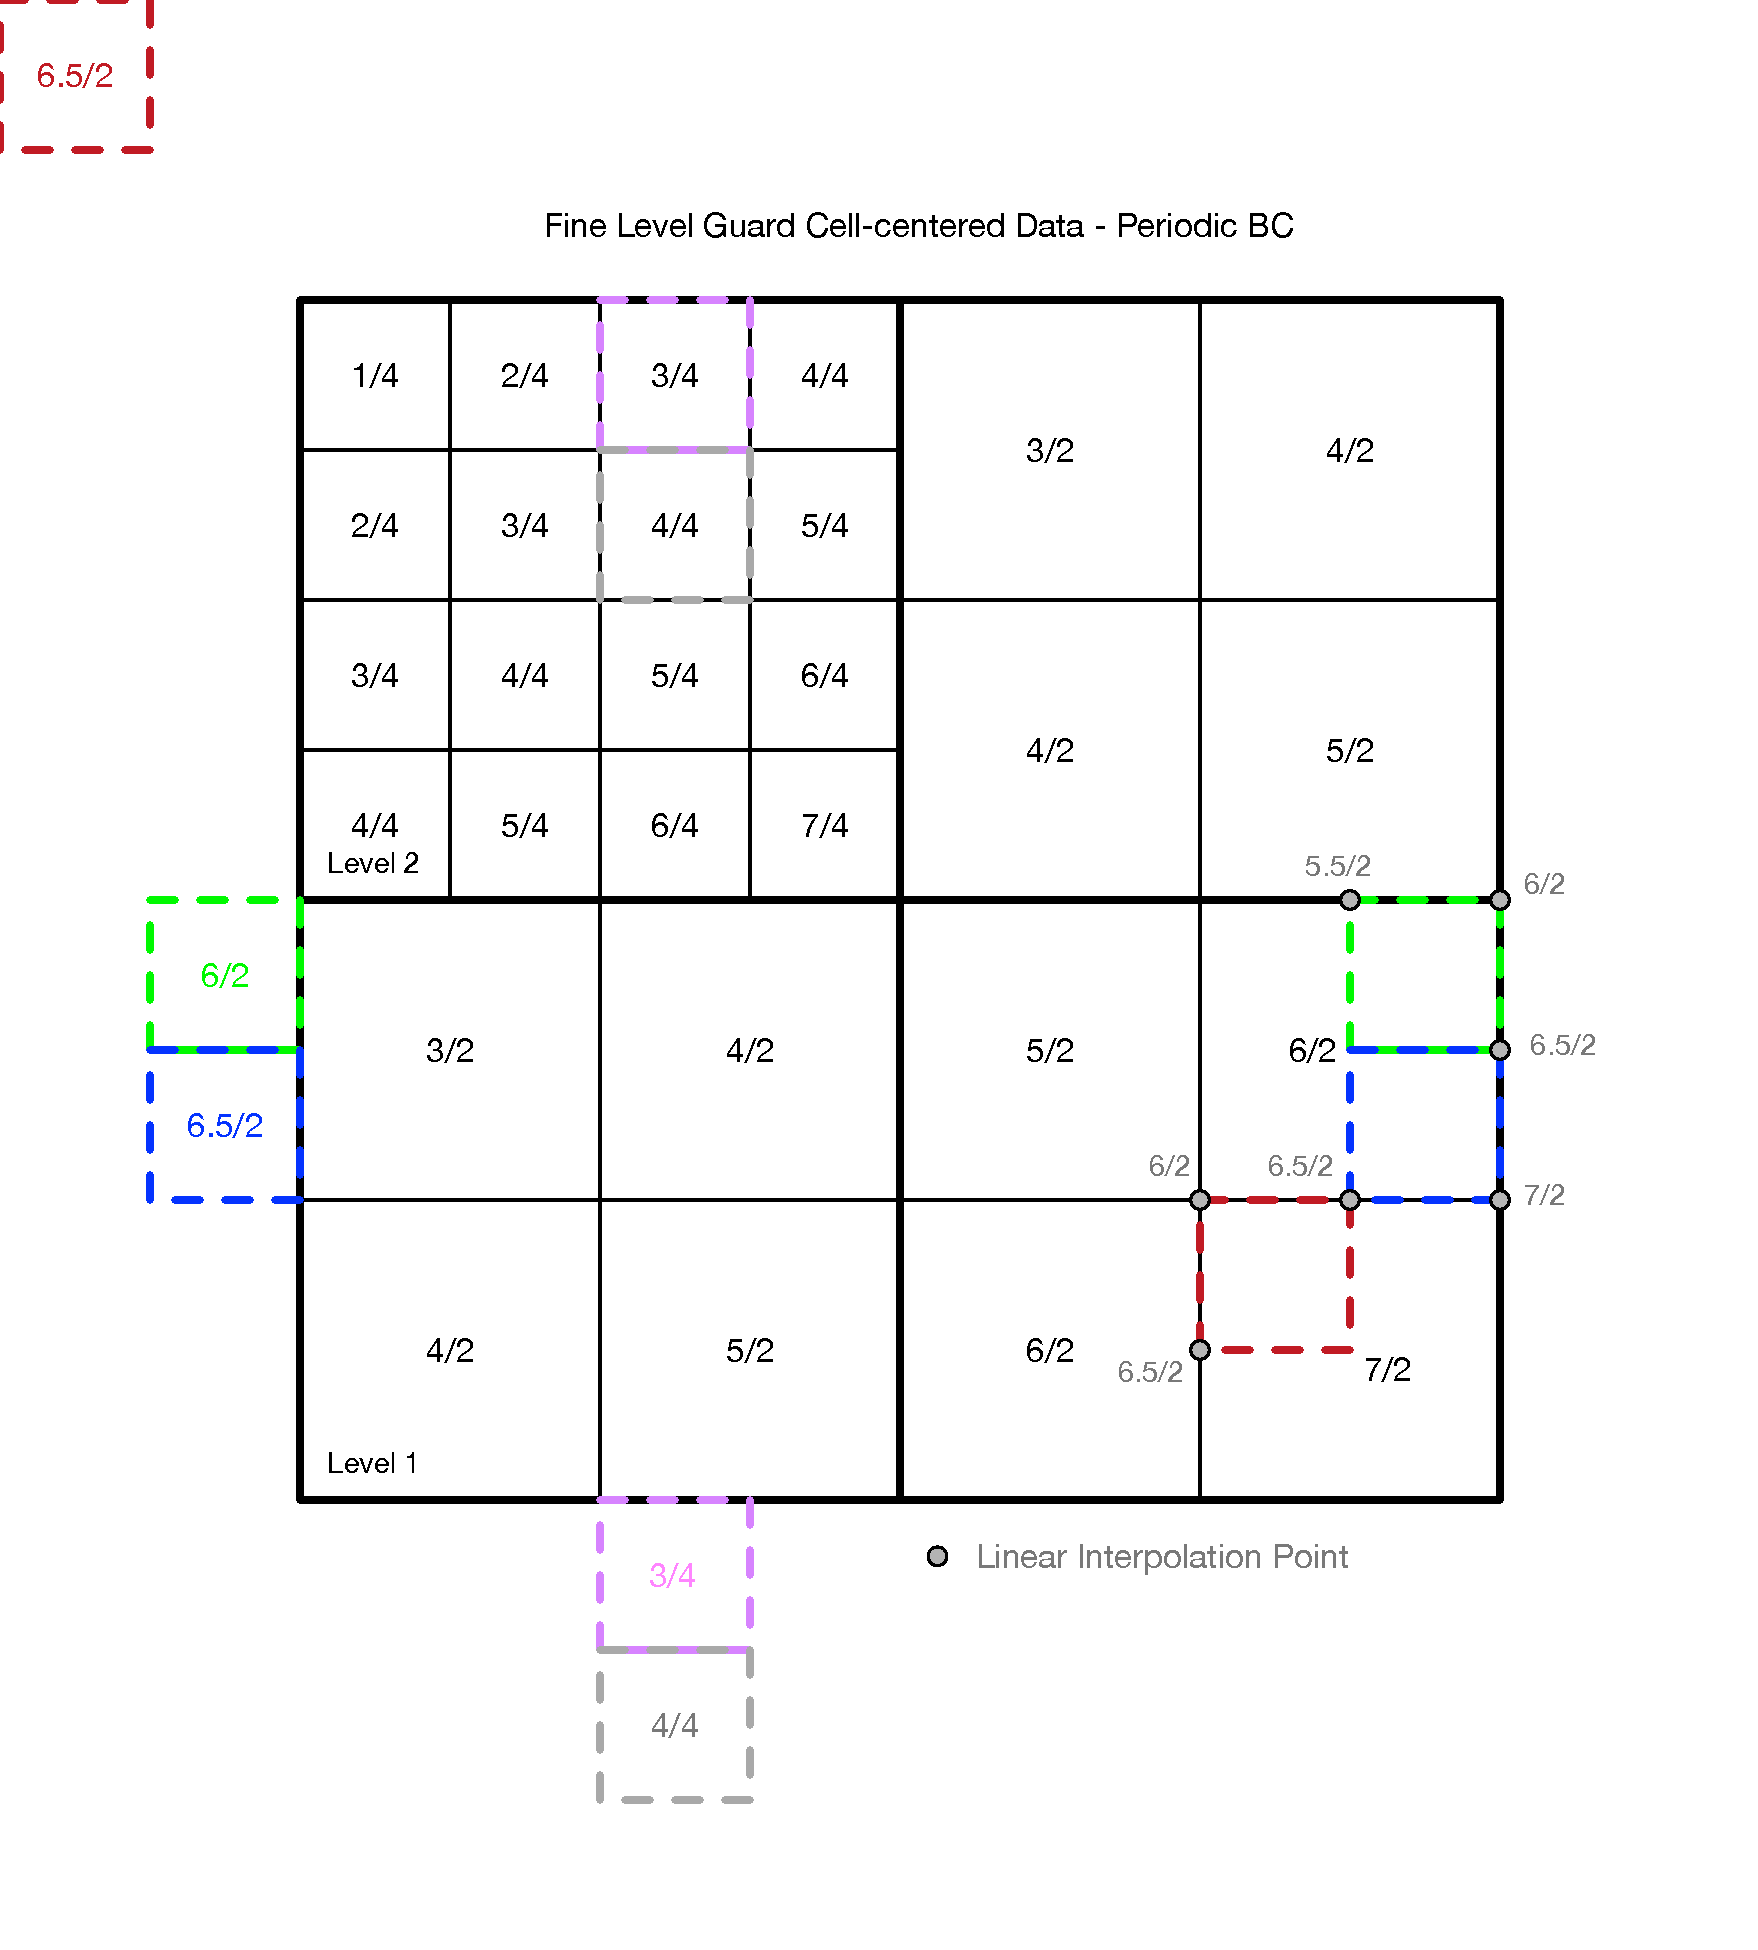
\includegraphics[width=6.5in]{TestGcFill_FineGC.pdf}
\caption{Spot check some cell-centered guardcell data in Level 2.}
\end{center}
\end{figure}

\end{document}

